\documentclass{article}
\usepackage{CJKutf8, indentfirst, graphicx, subfigure}
\begin{document}
\begin{CJK}{UTF8}{bsmi}
\title{硬體設計與實驗 Lab2 Report}
\author{
104021219 鄭余玄
}
\date{}
\maketitle
\section{實做過程}
這次的 lab 我都是使用 behavioral 描述方式撰寫的,因此能比較簡潔地完成。
lab2\_1 我是先判斷一些邊界條件,像是 enable 是 0,或是大於 9 的輸入,剩下的對照 BCD 規格,並稍做整理,再使用 if 做條件判斷,就能夠簡單地完成實做了。

lab2\_1\_t 是 lab2\_1 的 testbench,
因為要求要測試過所有可能的輸入和輸出,
所以我使用 repeat 把所有組合都跑遍。
同時也運用到上課教的 task 語法,
重複使用助教之前的 printerror task 來輸出錯誤。
此外,我比較不偏好用助教計算 delay 時間的方式來控制測試訊號,
因為一旦程式碼區塊執行順序有變更的時候,
每次都需要手動再計算一次執行的時間,
這會減少了程式碼的可變性。

lab2\_2 多虧助教已經先畫好了 block diagram,
看著圖和對照規格再把線路接上就完成了。
再加上助教已經寫好測試,
所以很快就完成了!

\subsection{Block diagram}
\begin{figure*}[h]
\centering{
\hfill
  \subfigure[]{ \label{fig:sub1}
  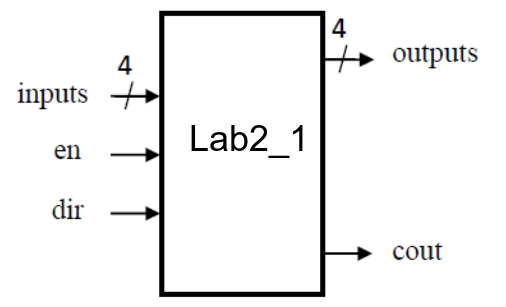
\includegraphics[width=.4\textwidth, angle=0]{lab2_1}
}
\hfill
  \subfigure[]{ \label{fig:sub2}
    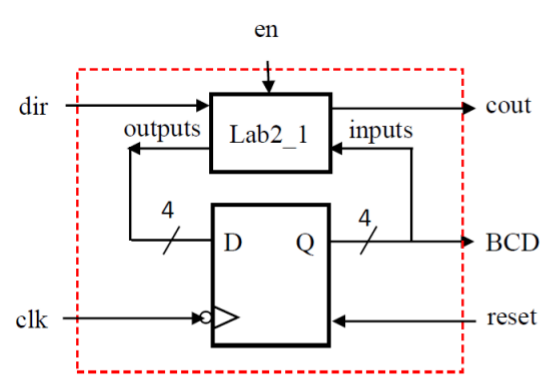
\includegraphics[width=.4\textwidth, angle=0]{lab2_2}
  }
\hfill
}
\caption{Block diagrams: (a) BCD and (b) 1-digit BCD up/down counter.}
\end{figure*}
這次的 block diagram 基本上助教都已經提供好了,尤其是圖 \ref{fig:sub2},讓我在寫 code 時加快許多。
\section{心得}
這次在寫程式時,有一點粗心大意。
像是 lab2\_1 當初在跑第一次測試時居然沒有通過,
原因是在 dir = 0 時,有一段程式碼是複製 dir = 1 的,
不過忘了改運算,所以沒有通過測試。
幸好 lab2\_2\_t 的 dir = 0 的那段測試是手打的,
而不是複製 dir = 1那段測試的,
否則測試可能永遠測不出來了。

另外, lab2\_2 一開始也是有遇到錯誤,
不小心把判斷成 reset == 0 (應該是 reset == 1 才重設),
但是利用 error 編號,
就可以知道是在 test 中哪些  if 條件式判斷出錯誤,
就能夠反向追蹤回可能發生錯誤的原因了。
這次 lab 讓我感受到預防真的勝於治療,
多寫一個 bug,debug 時間就會多好幾倍。
\end{CJK}
\end{document}